%PHOIBLE pour PHOnetics Information Base and LExicon
\chapter{Association entre le /r/ trillé et la \textg{rugosité}} \label{chap:roughness}
\epigraph{\href{https://www.youtube.com/watch?v=Iary3X3Vyp0}{альвеолярный дрожащий}}

%Quelles questions posent le chapitre de Roughness ?
%Est-ce que malgré la faible occurence des trills, on peut expliquer de justifier leur présence dans les langues du monde ?
%Est-ce qu'il y a une motivation à continuer à utiliser \textg{trill} comme label descriptif ?

Le trill est un segment avec des caractéristiques singulières, qui le rendent intéressant pour les études de symbolisme sonore. Pour autant, comme ce segment est difficile à maîtriser à cause de sa représentation, il devient crucial de s'interroger sur les méthodes utilisées dans ce type d'études. Dans ce chapitre, nous allons répliquer une étude cross-linguistique intégrée à un article publié en 2022 en Open Access. Nous proposons un codage différent des données, en nous basant sur les informations apportées par des grammaires linguistiques. Ce chapitre s'articule avec le chapitre suivant, qui s'intéressera au travail des linguistes de terrain. Il cherchera à comprendre ce qui peut être inféré des grammaires à partir du corpus collecté pour cette réplication et des inventaires phonémiques en ce qui concerne le \textit{r}.

\begin{figure}
	\centering
	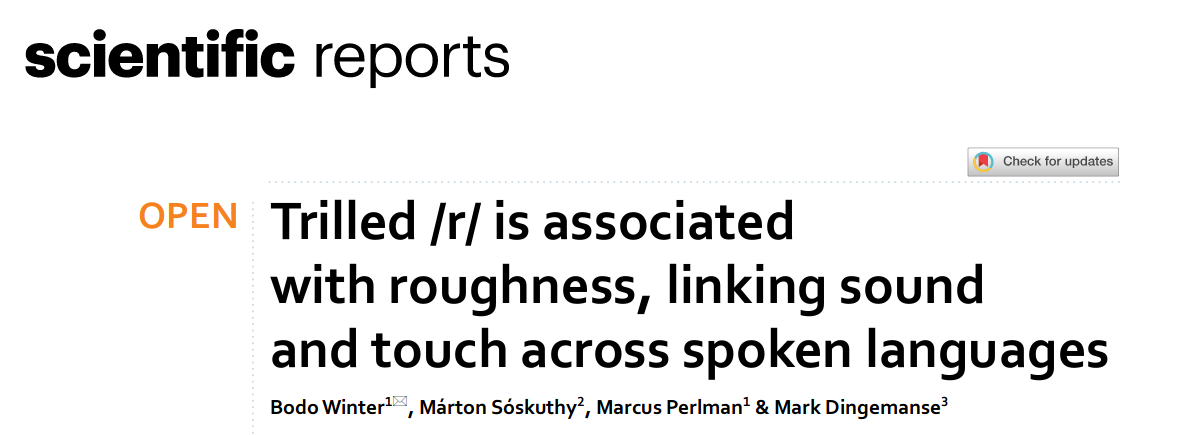
\includegraphics[width=1\linewidth]{substance/images/trilled_r}
	\caption[Titre de l'article de Winter et al. (2022) publié en Open Access]{Article de Winter et al. (2022) publié en Open Access dont nous avons cherché à répliquer l'étude cross-linguistique}
	\label{fig:trilledr}
\end{figure}

\section{Présentation de l'article de \textcite{winterTrilledAssociatedRoughness2022}}

L’article publié en Open Access intitulé \textit{Trilled /r/ is associated with roughness, linking sound and touch across spoken languages} [le /r/ trillé est associé avec la rugosité, liant son et touché à travers les langues orales] de Bodo Winter, Márton Sóskuthy, Marcus Perlman et Mark Dingemanse  \parencite*{winterTrilledAssociatedRoughness2022} (Figure \ref{fig:trilledr}) cherche à montrer qu’il peut exister une association iconique entre la texture rugueuse et le trill /r/.
À travers quatre études, les auteurs mettent en évidence ce qu’ils considèrent comme un universel statistique : les langues qui possèdent un /r/ trillé ont tendance à utiliser un mot pour la rugosité contenant ce type spécifique de /r/ par rapport aux autres langues sans /r/ trillé.\\

L'article développe trois études sur des langues indo-européennes et ouraliennes. L'association entre le \textg{trill} et la \textg{rugosité} est démontrée pour les adjectifs en anglais et en hongrois. Le proto-indo-européen permet de montrer que cette association s'allie à un signal fort dans la langue reconstruite. Ces trois études sont complétées par une étude à visée typologique à large échelle, ayant pour objet d'étude le lien entre iconicité et son dans 332 langues appartenant à 84 familles de langues. C'est cette étude que nous répliquons en proposant un re-codage des données.\\

La publication se compose de l’article qui inclut les résultats mais aussi la méthodologie, et des documents annexes (\textit{supplementary materials}) qui peuvent être retrouvés dans un \href{https://osf.io/6nma2/}{dossier OSF (Open science framework)\footnote{Disponible sur : \url{https://osf.io/6nma2}}} incluant les données utilisées ainsi que du code pour la préparation des données et les analyses finales. C'est sur la base de ces informations que nous répliquons l'analyse de \textcite{winterTrilledAssociatedRoughness2022}.\\

L'étude typologique s'appuie sur des bases de données lexicales. Les auteurs ont extrait des mots correspondant au sens de \textsc{rough} et \textsc{smooth} dans diverses bases de données (Google Traduction; RefLex; Chirila et CLICS). Ils ont ensuite constitué deux groupes pour faire leurs analyses.\\

Le premier groupe est celui des langues qui ont un /r/ trillé et aucune autre rhotique dans l’inventaire de la langue, et le deuxième groupe est celui des langues qui n’ont pas de /r/ trillé mais ont une autre rhotique dans leur inventaire.
En opposition, deux catégories de langues ont été exclues des analyses car les auteurs ont adopté une approche qu’ils qualifient de \textg{conservative} : celle des langues qui n’ont pas de rhotique, et celle des langues qui ont au moins deux rhotiques dont une qui est un /r/ trillé et l’autre qui est une rhotique non trillée.\\

Leurs décisions se basent sur PHOIBLE \parencite{phoible} et sur leurs propres jugements phonétiques liés aux descriptions existantes des langues dans les grammaires descriptives, les articles, l'encyclopédie collaborative en ligne Wikipédia ou des sites web spécialisés.
Ce sont 179 langues avec un trill /r/ et 153 langues avec une autre rhotique qui ont été incluses dans l'étude cross-linguistique.

\section{Qu'est-ce qu'un /r/ trillé ?}

L'affirmation de \textcite{winterTrilledAssociatedRoughness2022} est forte et repose sur des postulats méthodologiques dont on peut questionner la solidité. Les résultats de nos réflexions se basant sur la littérature ainsi que nos précédentes analyses (cf. \autoref{chap:jipa} et \autoref{chap:acoustics}) nous ont montré que caractériser le trill n’est pas une tâche évidente à cause de sa variation. 
Les \textit{supplementary materials} comprennent une liste de segments considérés comme trill et autre. Ainsi, les auteurs ne définissent pas ce qu'ils considèrent comme un /r/ trillé autre que par le caractère \textit{r} et semblent ignorer la variation associée aux rhotiques. 
La frontière entre phonétique et phonologie est souvent brouillée en linguistique descriptive \parencite{maddiesonPhoneticAdequacyDescriptive2021}. L'utilisation de dictionnaires est adéquate pour observer les éléments contrastifs phonémiques d'une langue, mais n'est pas très informative sur la valeur phonétique de ces segments. De l'information peut être perdue à cause d'orthographes standardisées \parencite[130]{riceIssuesStandardizationCommunity2002}. Pour cette raison, nous avons voulu répliquer, en recodant les données, l'étude cross-linguistique de \textcite{winterTrilledAssociatedRoughness2022} avec une analyse fine des données issues de grammaires.
Ainsi, nous souhaitons savoir si notre réplication entraînera un jeu de données différent, et si les mêmes conclusions pourront être atteintes.
De même que les auteurs, nous ne connaissons les langues incluses dans l'analyse que par l'intermédiaire des ressources disponibles dans les bibliothèques ou sur Internet. Nos connaissances des langues ne sont que partielles.
\href{https://soskuthy.github.io/}{Márton Sóskuthy} a été principalement en charge de la collection et de la préparation des données. Il est l'auteur d'une \href{https://era.ed.ac.uk/handle/1842/8946}{thèse} \parencite{soskuthyPhoneticBiasesSystemic2013} sur les biais phonétiques et les effets systémiques dans la mise en œuvre d'un changement sonore à travers des modèles computationnels.\\

Dans ce chapitre, dans un premier temps, nous allons détailler la méthodologie utilisée pour investiguer de manière systématique, chaque langue incluse dans les données d'origine.
Il s'agit de trouver des ressources pour déterminer si les langues possèdent ou non un /r/ trillé dans leur inventaire de sons, ce qui n'est pas simple.
Nous avons pris en compte uniquement les informations que nous avons pu récolter et non nos propres intuitions. Certaines langues qui avait été codées avec un /r/ trillé ne possèdent pas de /r/ trillé.
Pour plusieurs langues, il est impossible d'affirmer la présence de /r/ trillé.
D'autres langues ont été catégorisées comme ne possédant pas de /r/ trillé alors que c'était le cas.
Le re-codage des données sert à mettre en évidence la complexité de la caractérisation de la rhotique d'une langue par un symbole et un label descriptif, et des inférences qui peuvent exister.\\
Dans un second temps, nous présentons les résultats de la réplication de l'analyse de l'article original avec le même code, les mêmes paramètres des modèles statistiques. Nous mettrons en évidence que, bien que l'association entre \textg{rugosité} et \textg{trill} existe, elle n'est pas limitée à ce type de segment, mais existe pour toutes les rhotiques.


\section{Collection des données primaires et re-codage des langues}

\begin{figure}
	\centering
	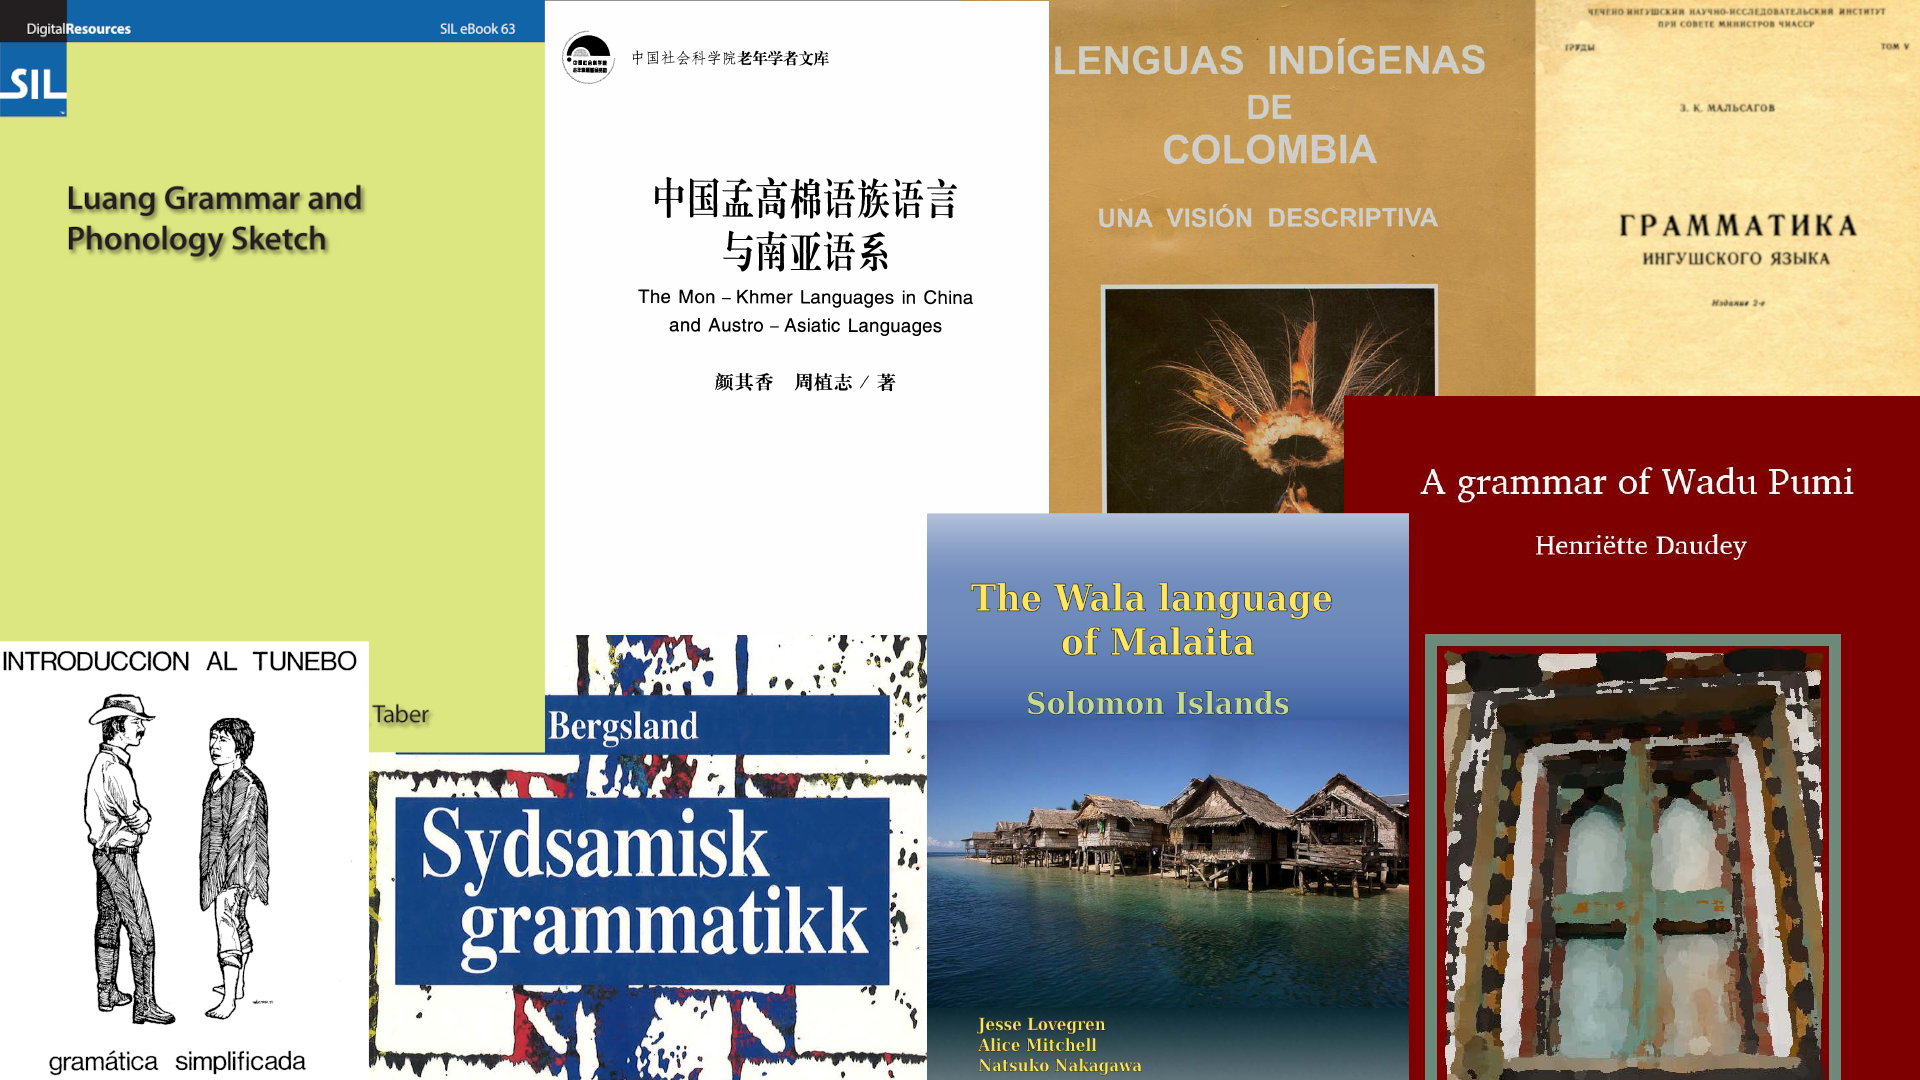
\includegraphics[width=1\linewidth]{substance/images/corpus_leng}
	\caption[Collage de couvertures d'ouvrages linguistiques décrivant des langues]{Collage de couvertures d'ouvrages linguistiques décrivant des langues. Ces premières de couverture, toutes très différentes, nous apparaissent comme mettant en avant la diversité des cultures et des traditions linguistiques.}
	\label{fig:corpusleng}
\end{figure}

Nous avons récupéré toutes les données disponibles et accessibles à partir de la littérature existante sur les langues d'intérêt.
Nous avons comparé et intégré plusieurs informations pour comprendre la classification faite par les auteurs et proposer un re-codage des données lorsque nous n'étions pas d'accord avec les auteurs. La recherche d'informations s'est faite généralement à travers les ouvrages référencés par \href{https://glottolog.org/}{Glottolog.org}. Ces ouvrages sont de différentes natures. On retrouve des grammaires plus ou moins longues, des esquisses grammaticales, ou encore des ouvrages de phonologie décrivant l'inventaire de sons de la langue à travers des paires minimales \parencite{hammarstromSimultaneousVisualizationLanguage2018}.
Pour les grammaires et les esquisses grammaticales, les informations ont principalement été extraites des chapitres de phonétique et de phonologie, que nous appelons les chapitres de \textg{phonético-phonologie}.\\


Dans le but de procéder à la même recherche d'informations dans les ouvrages, nous avons rassemblé des informations spécifiques à plusieurs niveaux. Un premier niveau de recherche a été de prendre en compte les observations et le codage de \textcite{winterTrilledAssociatedRoughness2022} que nous avons mis en perspective avec un deuxième niveau d'analyse correspondant aux informations collectées dans la littérature scientifique et sur des ressources en ligne.

Pour chaque langue, nous avons les catégories suivantes :

\begin{itemize}
	\item Trill : La valeur accordée par \citeauthor{winterTrilledAssociatedRoughness2022} à la présence du trill : \texttt{yes} ou \texttt{no}. La valeur est binaire.\\
		Le \texttt{yes} correspond à la présence du trill.\\
		Le \texttt{no} correspond à présence d'une autre rhotique qui n'est pas trillée.\\
		Ces deux valeurs sont issues des informations extraites de PHOIBLE (cf. R\_type) et des recherches de \citeauthor{winterTrilledAssociatedRoughness2022} sur les langues.
	\item R\_type : La valeur se basant principalement sur les inventaires de PHOIBLE récupérés automatiquement par les auteurs. On retrouve quatre valeurs possibles : \texttt{trill}, \texttt{no trill}, \texttt{mixed with trill} ou \texttt{no rhotic}.\\
	Le \texttt{trill} correspond à la présence du \textit{r}.\\
	Le \texttt{no trill} correspond à l'absence du \textit{r} mais à la présence d'un autre symbole pour une rhotique.\\
	Le \texttt{mixed with trill} correspond à la présence du \textit{r} et à la présence d'un autre symbole pour une rhotique.\\
	Le \texttt{no rhotic} correspond à l'absence du \textit{r} et à l'absence d'un autre symbole pour une rhotique.
\end{itemize}

Le codage des auteurs permet de ne pas avoir de langues sans rhotique dans l'analyse. Seules les langues avec des <r> sont incluses. De surcroît, le codage des auteurs permet d'exclure les langues avec deux rhotiques contrastives, dont l'une est un trill.
Dans certains cas, la valeur de la catégorie \textg{Trill} était différente de celle de la catégorie \textg{R\_type}. Lors de ce type de conflit de valeurs, les auteurs ont fait le choix de prendre la valeur de la catégorie \textg{Trill}. Cette dernière se veut plus fiable car elle est issue d'une vérification manuelle.\\

Nous avons ajouté d'autres informations issues des données en \textit{supplementary materials} des auteurs :

\begin{itemize}
	\item Dataset : La base de données d'où proviennent les mots pour les concepts \textsc{rough} (\textg{rugueux}) et \textsc{smooth} (\textg{lisse}). On retrouve cinq bases de données lexicales : \href{https://translate.google.com/?hl=fr&sl=auto&tl=en&op=translate}{Google Traduction\footnote{Disponible sur : \url{https://translate.google.com}}} pour les langues qui sont relativement bien documentées, \href{https://reflex.cnrs.fr/Africa/}{RefLex\footnote{Disponible sur : \url{https://reflex.cnrs.fr/Africa}}} (pour les langues parlées en Afrique), \href{http://chirila.yale.edu/}{Chirila\footnote{Disponible sur : \url{http://chirila.yale.edu}}} (pour les langues parlées en Australie), \href{https://ids.clld.org/}{IDS\footnote{Disponible sur : \url{https://ids.clld.org}}} [The Intercontinental Dictionary Series]  et \href{https://clics.clld.org/}{CLICS\footnote{Disponible sur : \url{https://clics.clld.org}}} [Database of Cross-Linguistic Colexifications].
	\begin{itemize}
		\item Nous avons en plus pris en considération les commentaires ajoutés par les auteurs pour justifier le choix de la rhotique dans la langue : ces commentaires pouvaient être un lien avec une source où l'articulation de la rhotique est caractérisée, une référence d'une grammaire ou d'un article publié, ou encore le renvoi vers Wikipédia.\\
		Lorsque le commentaire incluait une ou des référence(s), nous avons reporté l'information qui nous paraissait importante dans le but d'aller vérifier les informations sur les rhotiques.
	\end{itemize}
	\item PHOIBLE : Nous avons reporté manuellement le ou les symbole(s) utilisé(s) pour la ou les rhotique(s) de la langue ainsi que les allophones lorsqu'ils sont mentionnés, en fonction de l'inventaire répertorié par la base de données. Lorsqu'il y avait plusieurs inventaires pour une langue, nous avons vérifié chaque inventaire inclus dans PHOIBLE.
	\begin{itemize}
		\item Lorsque cela était possible, nous avons vérifié les sources primaires dans le nom des références citées par PHOIBLE d'où proviennent les segments.
	\end{itemize}
	\item Wikipédia : Nous avons reporté manuellement le ou les symbole(s) utilisé(s) pour la ou les rhotique(s) de la langue, lorsqu'il y avait un tableau des consonnes sur la page Wikipedia.
	\begin{itemize}
		\item Nous avons, de plus, reporté la description et/ou les commentaires associés aux segments d'intérêt disponibles sur la page Wikipédia.\\
		Nous avons regardé les sources du tableau consonantique lorsqu'elles étaient présentes, pour s'assurer que la page Wikipédia reportait avec exactitude la ou les source(s) primaire(s).
	\end{itemize}
	\item Glottolog : Nous avons reporté manuellement le lien vers la page \href{https://glottolog.org/}{Glottolog.org} associée au glottocode donné par les auteurs, où il est possible de retrouver une bibliographie pouvant inclure des descriptions grammaticales ou phonologiques.\\
	Pour certaines références, nous n'avions que la translittération du nom de la référence, ce qui a rendu difficile voire impossible la recherche de la référence dans certains cas.
	\item Autres sources : Nous avons reporté manuellement le lien vers d'autres sources avec leur contenus. Lorsque la base de données principale était CLICS, nous avons collecté les différentes représentations orthographiques qui pouvaient être utilisées pour la rhotique ainsi que la fréquence du segment dans le lexique avec une visée exploratoire.
\end{itemize}

%\begin{figure}
%	\centering
%	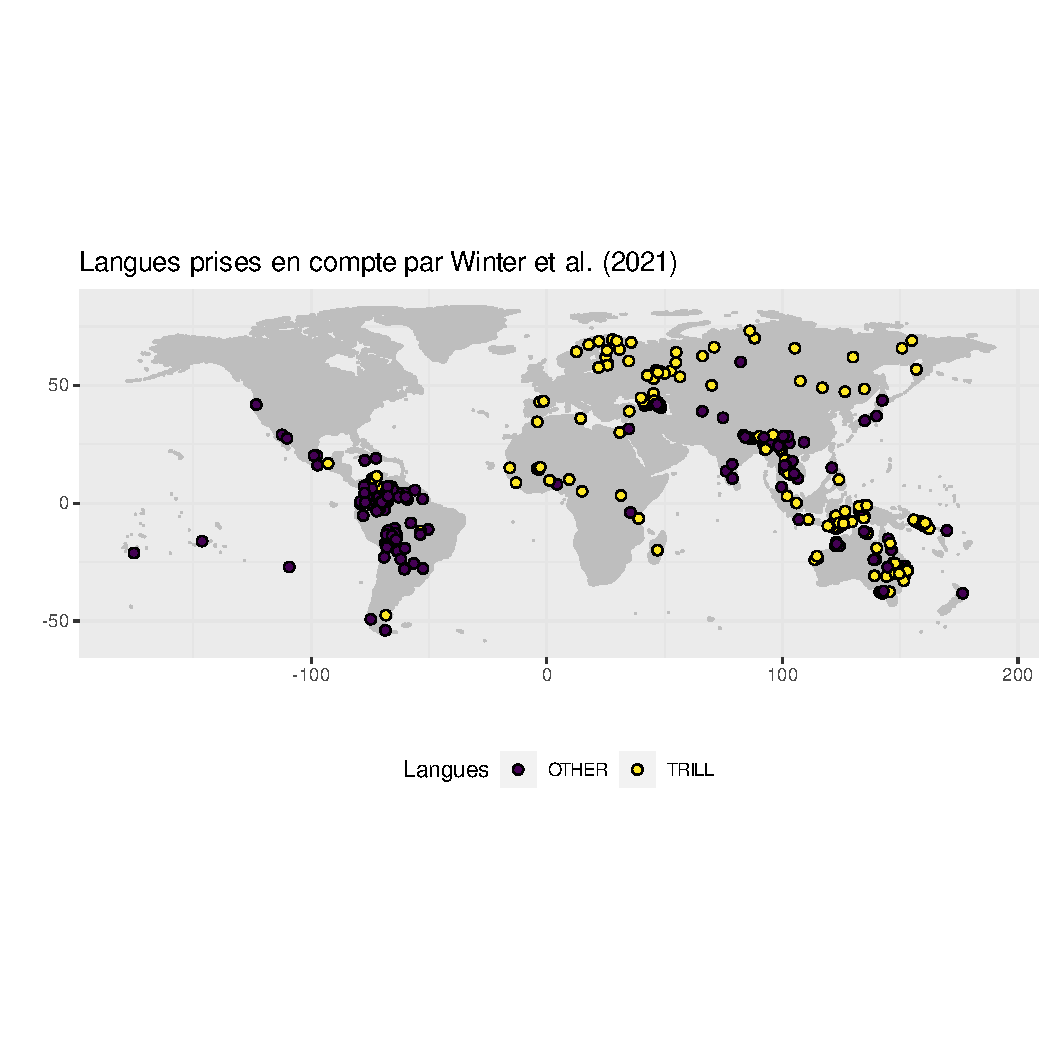
\includegraphics[width=1\linewidth,
%					trim={0 4.25cm 0 4.25cm}, clip]{substance/images/carte_winter_avant}
%	\caption[Distribution des langues incluses dans \textcite{winterTrilledAssociatedRoughness2022}]{Distribution des langues incluses dans l'analyse originale de \textcite{winterTrilledAssociatedRoughness2022}. Deux groupes sont inclus : les langues \textsc{trill} et les langues \textsc{other}. Les langues Indo-Européennes ne sont pas incluses.}
%	\label{fig:cartewinteravant}
%\end{figure}

%\begin{figure}
%	\centering
%	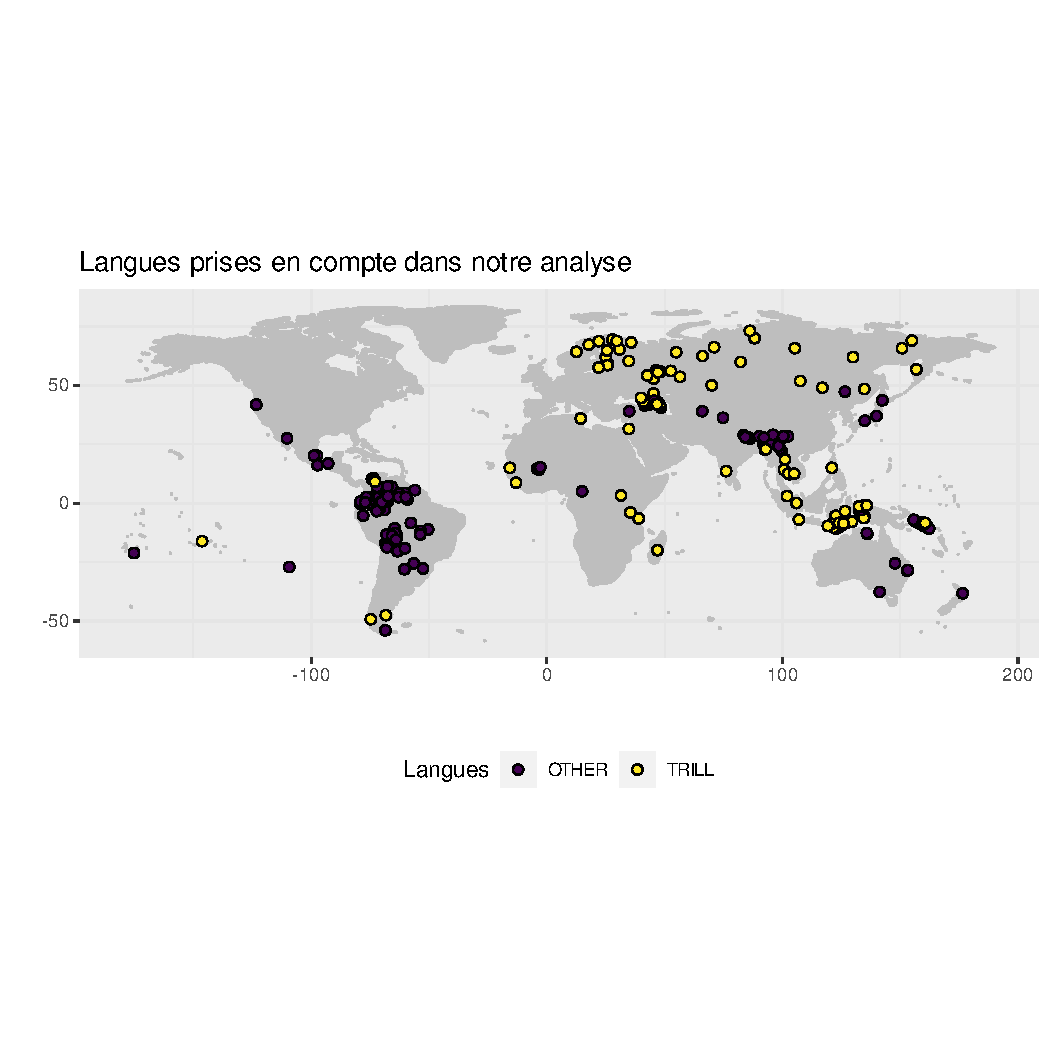
\includegraphics[width=1\linewidth,
%	trim={0 4.25cm 0 4.25cm}, clip]{substance/images/carte_winter_apres}
%	\caption[Distribution des langues incluses dans notre analyse]{Distribution des langues incluses dans notre analyse. Deux groupes sont inclus : les langues \textsc{trill} et les langues \textsc{other}. 76 langues, en plus des langues Indo-Européennes ont été exclues.}
%	\label{fig:cartewinterapres}
%\end{figure}

\subsection{Deux exemples de langues recodées}

Nous avons voulu illustrer le problème du codage des langues par deux exemples. La première langue, le tabasaran (dialecte du sud), a initialement été codée comme possédant un trill. Cependant, comme nous ne pouvions pas reproduire la méthodologie qui a abouti à ce codage, nous avons choisi d'exclure cette langue de notre analyse. La deuxième langue, le mosetén, a été codée comme possédant une rhotique autre, c'est-à-dire une rhotique qui n'était pas un trill. En cherchant dans les différentes références où la phonologie et la phonétique du mosetén sont mentionnées avec l'utilisation du terme \textg{trill}, nous avons choisi de re-coder cette langue comme ayant un trill. Nous pouvons maintenant détailler ces deux exemples.\\

Prenons comme premier exemple celui du \texttt{Tabasaran (Southern dialect)}. Le dialecte méridional du tabasaran est parlé en Russie, dans la région du Daghestan. Le tabasaran fait partie de la famille de langues  \href{https://glottolog.org/resource/languoid/id/nakh1245}{nakho-daghestaniennes}. Les mots pour \textsc{rough} et \textsc{smooth} proviennent de CLICS. L'inventaire des consonnes n'est pas disponible dans PHOIBLE.

Ce dialecte a été considéré par les auteurs comme ayant un /r/ trillé, cette décision a été faite sur la base des informations disponibles sur \href{https://en.wikipedia.org/wiki/Tabasaran_language}{Wikipédia\footnote{Dernier accès en août 2022 sur \url{https://en.wikipedia.org/wiki/Tabasaran_language}}}. En effet, dans le tableau consonantique présent sur la page, le \textit{r} est associé au label descriptif \textit{trill}. Sur Wikipédia, on retrouve comme source le site web \href{https://titus.fkidg1.uni-frankfurt.de/didact/caucasus/nekklaut.htm}{Thesaurus Indogermanischer Text- und Sprachmaterialien\footnote{Dernier accès en août 2022 sur \url{https://titus.fkidg1.uni-frankfurt.de/didact/caucasus/nekklaut.htm}}} [Trad. Thesaurus de textes et de matériaux linguistiques indo-européens] avec le tableau du système du tabasaran (\href{https://titus.fkidg1.uni-frankfurt.de/didact/caucasus/nekklaut.htm#XFN3}{The consonant system of Tabasaran}). Dans ce tableau, on ne retrouve aucune mention du label descriptif \textsc{trill}. À ce tableau est associée une source (А.А. Магометов, Табасаранский язык (Исследование и тексты), Тбилиси 1965 / {\fontspec[Scale = 0.85]{DejaVuSerif}ალ. მაჰომეტოვი, თაბასარანული ენა (გამოკვლევა და ტექსტები), თბილისი} 1965 / A.A. Mahometov, Tabasaranskij jazyk (Issledovanie i teksty), Tbilisi 1965, p. 55).
Nous n'avons pas retrouvé la source d'origine. Pour cela, nous avons consulté Табасаранский язык [Trans. Tabasaranskij Jazyk] de \textcite{alekseevm.e.TabasaranskiyYazyk2003}, source dans laquelle on retrouve le label descriptif Сонорные [Trad. Sonante] (p. 29). La grammaire parlant de gémination et de processus phonologique mettant en jeu deux segments identiques côte-à-côte, nous avons cherché dans \href{https://clics.clld.org/languages/ids-68}{CLICS\footnote{Dernier accès en août 2022 sur \url{https://clics.clld.org/languages/ids-68}}} les fréquences des séquences <r> et <rr>. <r> est associé à 677 occurrences contre 0 pour <rr>.%Алексеев М. Е. et Шихалиева С. Х.

À cause du manque d'information trouvable et d'évidence en faveur du \textit{trill}, nous avons décidé de ne pas considérer cette langue pour notre analyse, et elle a donc été exclue de notre liste de langues finale.\\

Prenons comme deuxième exemple le \texttt{Mosetén}. Le mosetén est un isolat de la famille du \href{https://glottolog.org/resource/languoid/id/mose1249}{Mosetén-Chimané} parlé en Bolivie. La langue a été classée par \textcite{winterTrilledAssociatedRoughness2022} comme n'ayant pas de trill. Les mots pour \textsc{rough} et \textsc{smooth} proviennent de \href{https://clics.clld.org/languages/ids-271}{CLICS\footnote{Dernier accès en août 2022 sur \url{https://clics.clld.org/languages/ids-271}}}. Il existe quatre inventaires inclus dans PHOIBLE. Le premier est issu de la collecte de données de Moran (2012). On y retrouve les symboles r et ɽ. Dans la source d'origine \parencite{sakelGrammarMoseten2004}, la linguiste mentionne le terme \textit{trill} à au moins deux reprises pages 24-25 \textg{I will discuss the consonants one by one with respect to the their [\textit{sic}] type of articulation, i.e. plosives, fricatives, affricates, nasals, trills and approximants.} et page 33 avec une section pour le segment : \textg{/r/ is a short trill. Usually, the tongue hits the gum ridge only once. It can appear at the beginning of the syllable [...] and at the end of the	syllable [...]. Some people pronounce /r/ as a retroflex flap [ɽ].}.

Les trois autres inventaires de PHOIBLE proviennent de SAPHON (\href{https://linguistics.berkeley.edu/saphon/en/inv/MosetenC.html}{Mosetén de Covendo}, \href{https://linguistics.berkeley.edu/saphon/en/inv/MosetenSA.html}{Mosetén de Santa Ana}, \href{https://linguistics.berkeley.edu/saphon/en/inv/Tsimane.html}{Tsimané}) où les rhotiques ont systématiquement été codées avec le symbole ɾ. Les trois langues prennent pour source l'article en syntaxe de \textcite{sakelMosetenChimaneArgument2011} où il est juste mentionné que dans les phonèmes consonantiques on retrouve /r/ (p. 539).
De ces inventaires de PHOIBLE, il resort que le \texttt{R\_type} est \texttt{no trill}. En effet, dans les fichiers \texttt{markdown} de préparation des données, pour décider la valeur de \texttt{R\_type} les auteurs ont classé les sources de PHOIBLE pour prendre en premier les inventaires qui venaient de SAPHON \parencite{saphon} au dépit de ceux qui venaient de la collection de \textcite{moran_etal2014}. Pour une langue à plusieurs inventaires, l'inventaire dans une source hautement classée sera toujours sélectionné avant ceux des sources moins bien classées.

\href{https://en.wikipedia.org/wiki/Chimane_language}{Wikipédia\footnote{Dernier accès en août 2022 sur \url{https://en.wikipedia.org/wiki/Chimane_language}}} mentionne le \textit{trill} comme label descriptif pour le \textit{r} sur la base de \textcite{sakelGrammarMoseten2004}.
Des différentes références mentionnées par \href{https://glottolog.org/resource/languoid/id/mose1249}{Glottogue}, nous n'avons trouvé que les deux mentionnées précédemment.

Au-delà de rapporter ce qui a été dit sur le mosetén, ce cas ouvre la discussion sur deux points. Le premier point est celui de l'interprétation possible faisable à partir de la grammaire de \textcite{sakelGrammarMoseten2004}. La linguiste mentionne le trill avec la description de quelque chose qui ressemble à un tap. Cependant, à cause du manque d'information, il n'est pas possible de réinterpréter autrement le segment que par un trill. Sachant qu'un nombre conséquent de rhotiques semble être produit avec un seul battement, on peut se demander pourquoi la linguiste a choisi de parler de trill.
Si une langue est incluse dans une famille de langues où les rhotiques sont généralement décrites comme des taps, 
que nous est-il possible d'interpréter sur la rhotique dans cette langue ?
La personne qui décrira la rhotique dans cette langue pourra être biaisée en faveur du terme \textit{trill}, plus générique, mais pourra aussi choisir de ne pas rendre compte de la variation (consciemment ou inconsciemment) en reprenant la terminologie utilisée pour les langues apparentées.
Il semble que le mode opératoire de SAPHON est de reprendre la terminologie des rhotiques en Amérique du Sud lorsqu'il n'y a qu'une rhotique dans la langue. Ainsi, les taps et flaps sont surreprésentés dans la base de données car c'est l'information aréale qui importe, au détriment de l'information spécifique apportée par chaque linguiste dans sa grammaire.

Par conséquent, au vu des différentes informations que nous avons pu collecter, nous avons pris la décision de considérer le mosetén comme une langue possédant un trill.\\

Ces exemples, associés à ces pistes de réflexion, permettent d'expliquer pourquoi il y a une différence d'interprétation entre \textcite{winterTrilledAssociatedRoughness2022} et notre recodage. La réflexion sur la place des sons dans les grammaires sera abordée plus en détail dans le \autoref{chap:metagram}.\\


Au total, ce sont plus de 650 documents de tous types %(340 fichiers (Review)+ 294 fichiers (Review2) = 634) sans inclure les illustrations of the IPA ou les articles/livres qui étaient déjà dans mon Zotero. 
(\autoref{fig:corpusleng}), qui ont été utilisés pour procéder au recodage des données.

 \subsection{Résultats du recodage}

\begin{figure}
	\centering
	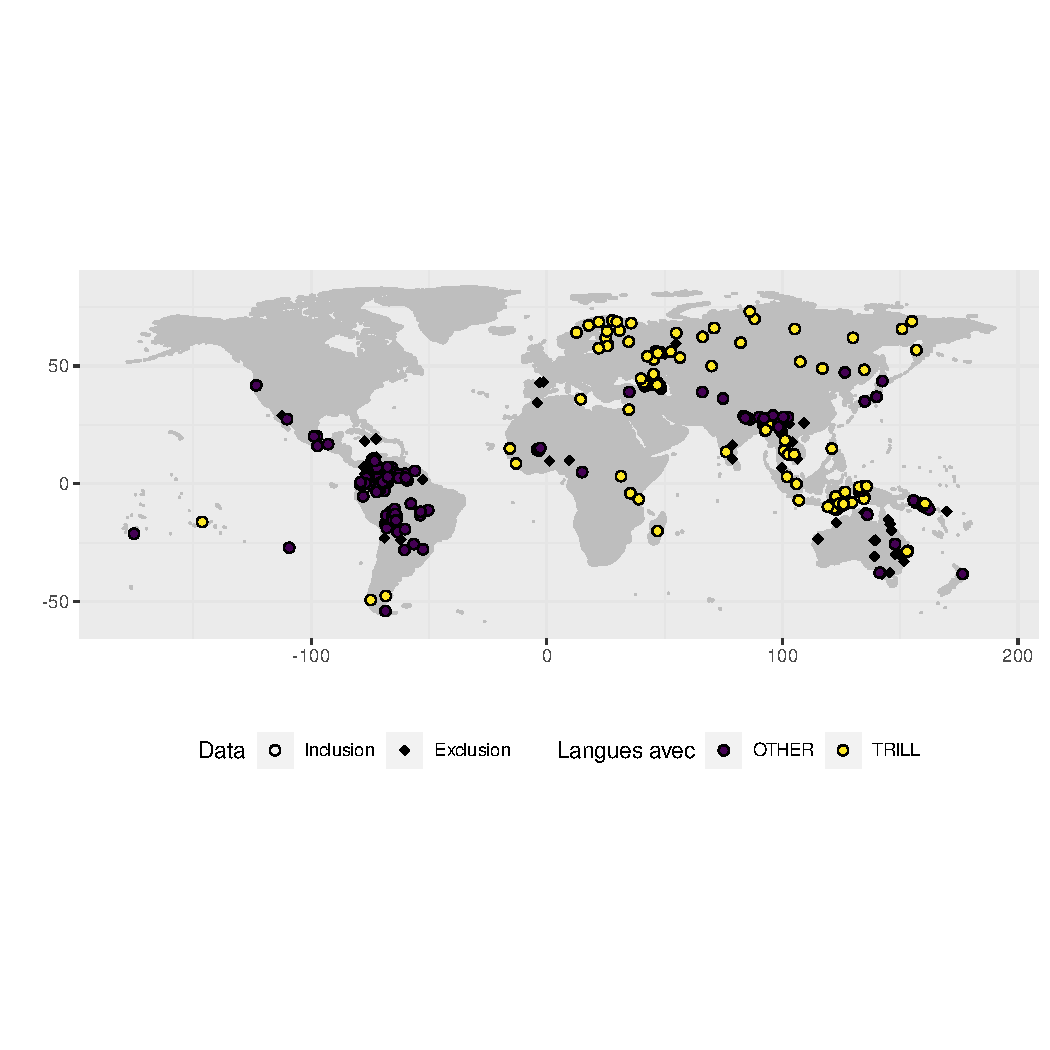
\includegraphics[width=1\linewidth, trim={0 4.75cm 0 4.5cm},clip]{substance/images/our_map_fr}
	\caption[Distribution des langues incluses dans \textcite{winterTrilledAssociatedRoughness2022}]{Distribution des langues incluses dans l'analyse originale de \textcite{winterTrilledAssociatedRoughness2022}. Deux groupes sont inclus : les langues \textsc{trill} et les langues \textsc{other}. Les langues Indo-Européennes ne sont pas incluses.}
	\label{fig:ourmapfr}
\end{figure}

L'analyse originelle comportait 332 langues (\autoref{fig:ourmapfr}). De ces langues nous n'en avons gardé que 256 pour 70 familles de langues après notre recodage (\autoref{fig:gramms}). Cette diminution dans le nombre de langues s'explique par l'exclusion de langues pour lesquelles nous n'avions pas d'information sur l'articulation de la rhotique, ou de langues qui auraient dû être exclues de l'analyse originelle de \textcite{winterTrilledAssociatedRoughness2022} car possédant un contraste entre deux rhotiques dont une trillée et une non-trillée, ou d'autres raisons comme le fait que la rhotique ne soit pas native de la langue.

\begin{figure}
	\centering
	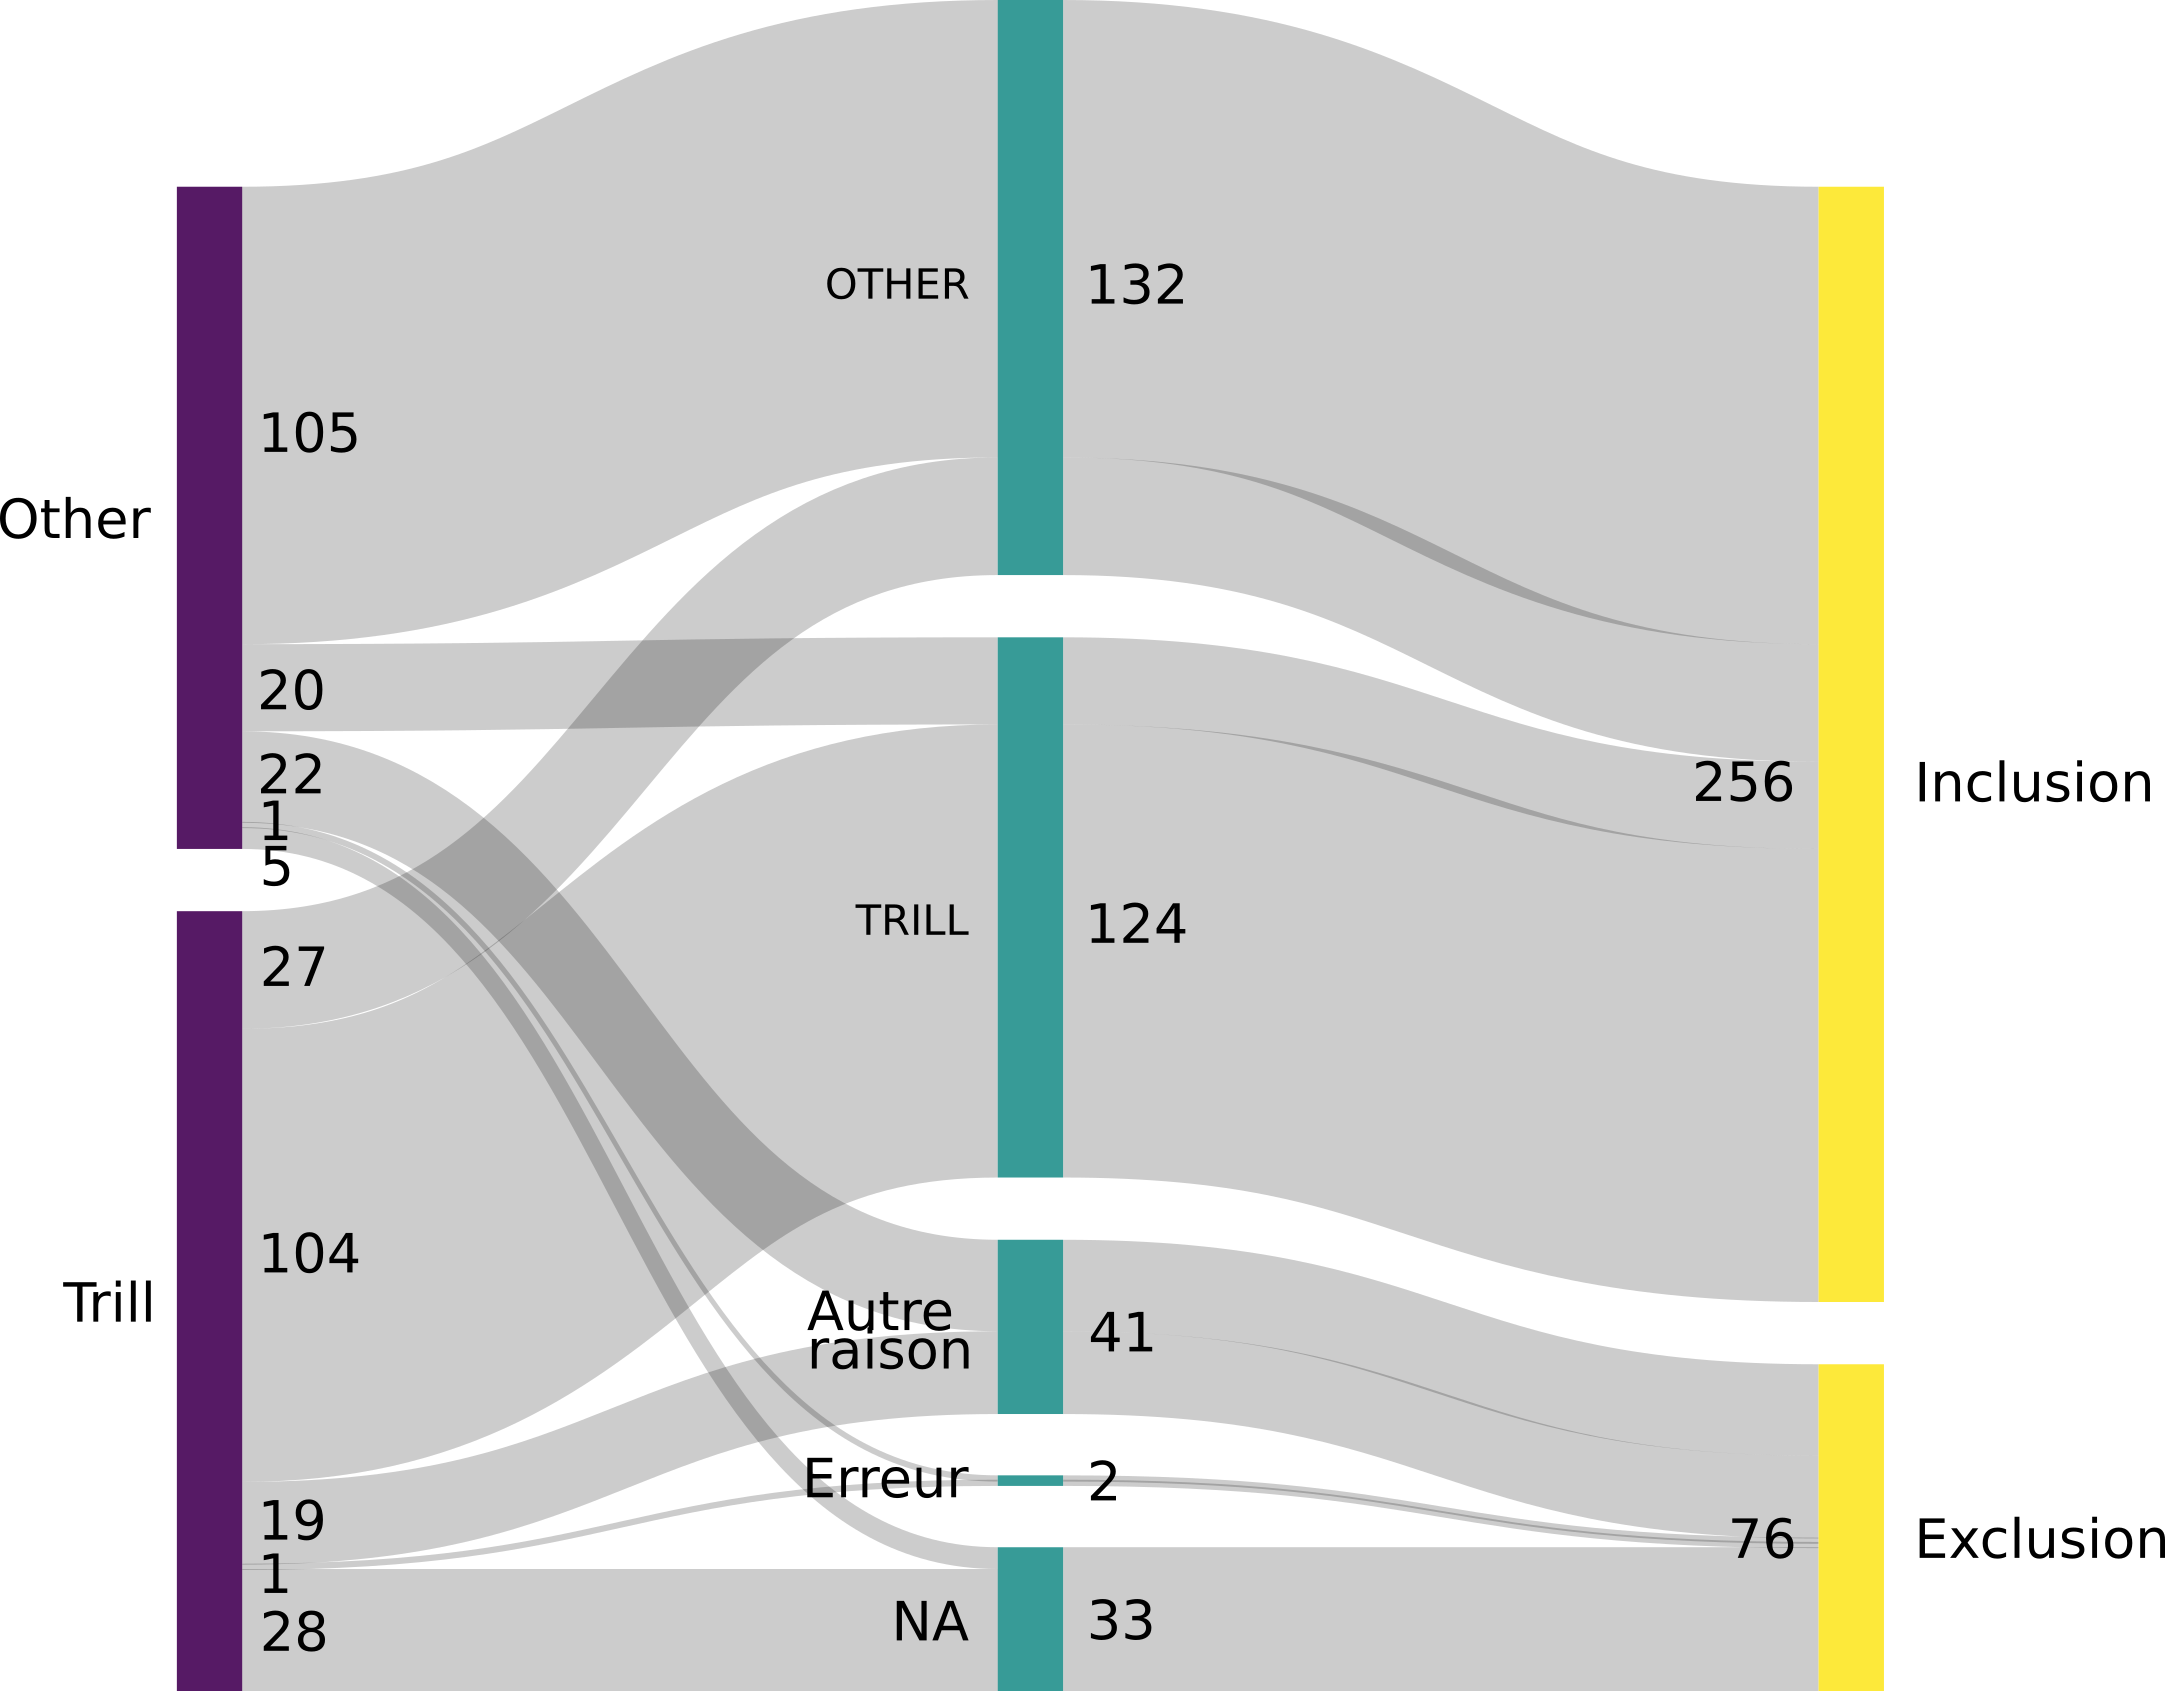
\includegraphics[width=1\linewidth]{substance/images/gramms}
	\caption[Diagramme illustrant le re-codage des langues en fonction des informations collectées]{Diagramme illustrant le re-codage des langues en fonction des informations collectées. À gauche le compte des langues telles que codées par \citeauthor{winterTrilledAssociatedRoughness2022}, au milieu les conclusions de notre processus de révision des valeurs de trill/other dans les langues, à droite le compte des langues inclues ou exclues dans notre réplication.}
	\label{fig:gramms}
\end{figure}


\section{Analyses et résultats}

\begin{figure}
	\centering
	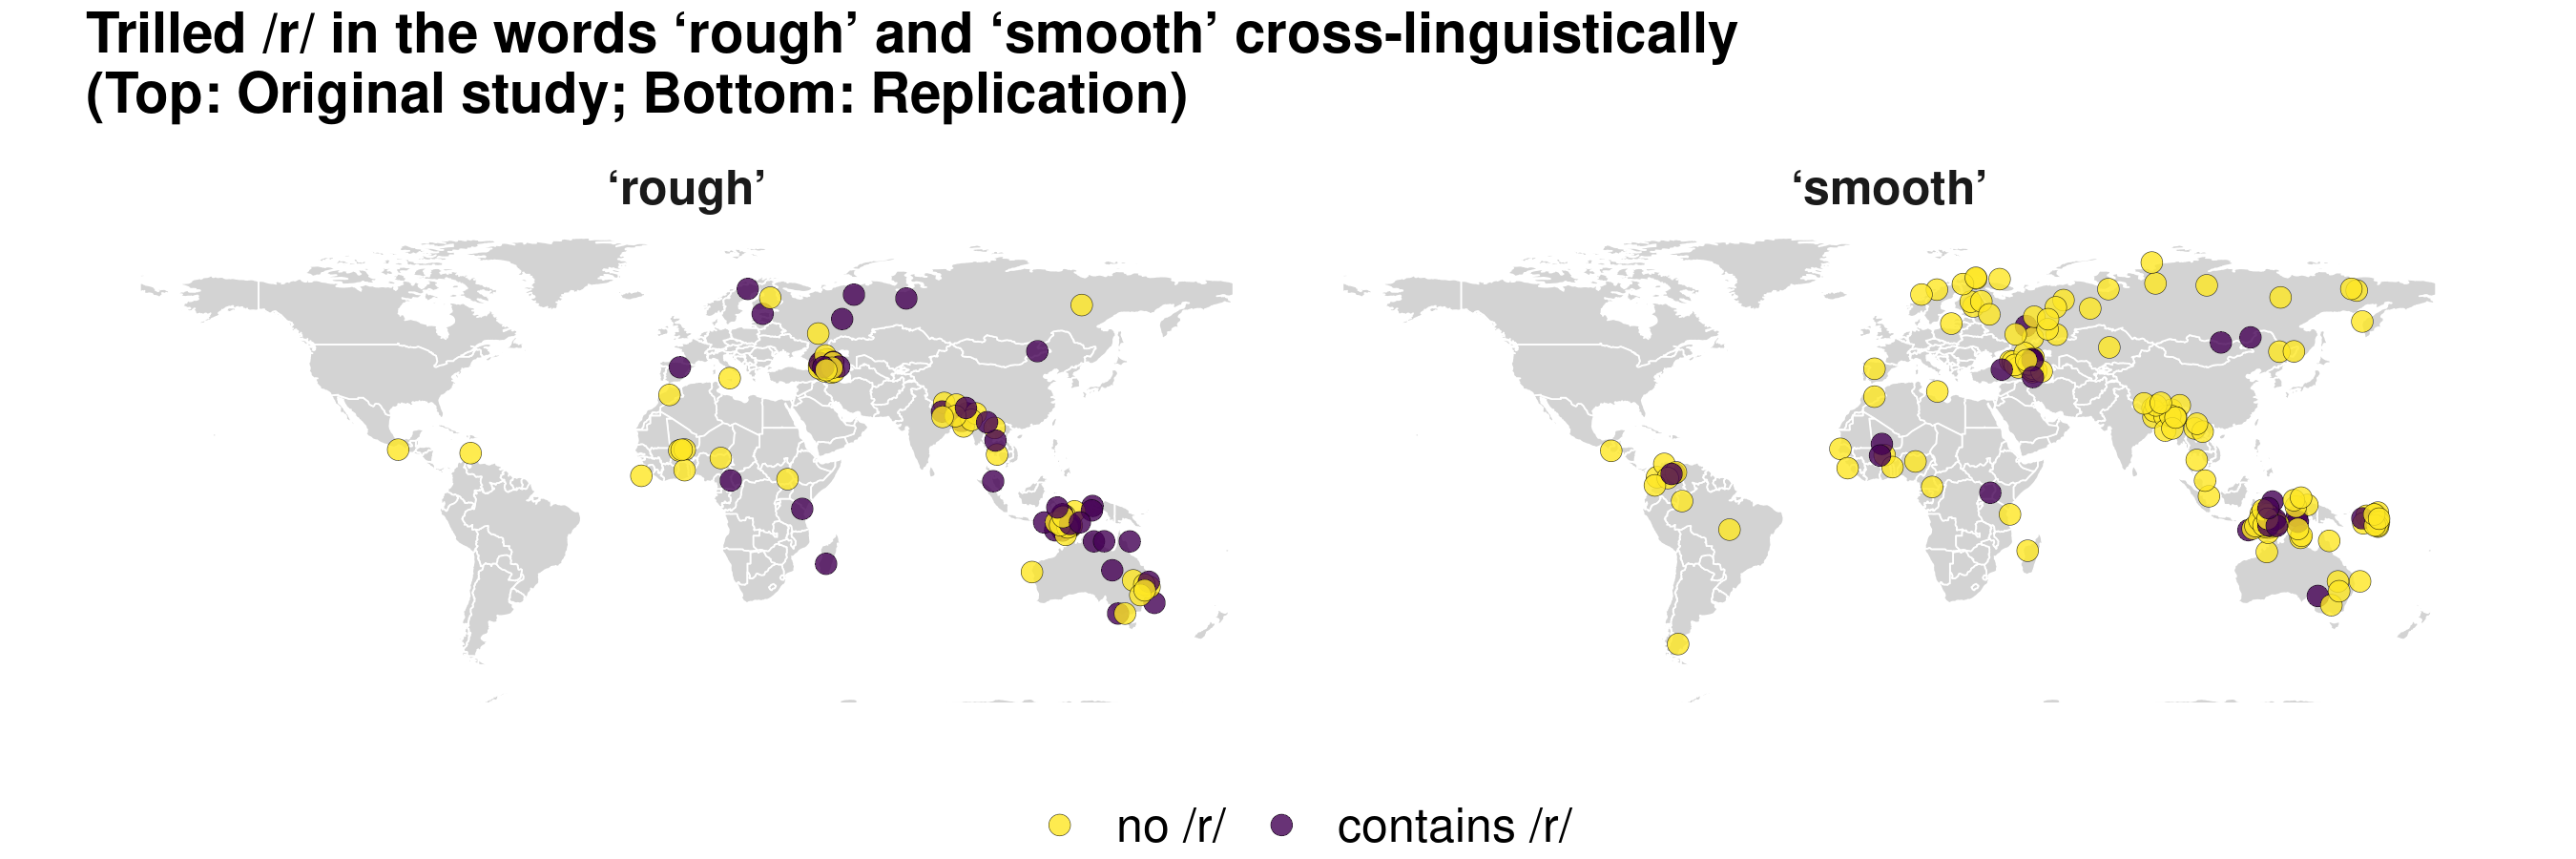
\includegraphics[width=1\linewidth, trim={0 0 0 0},clip]{substance/images/xling_map}
	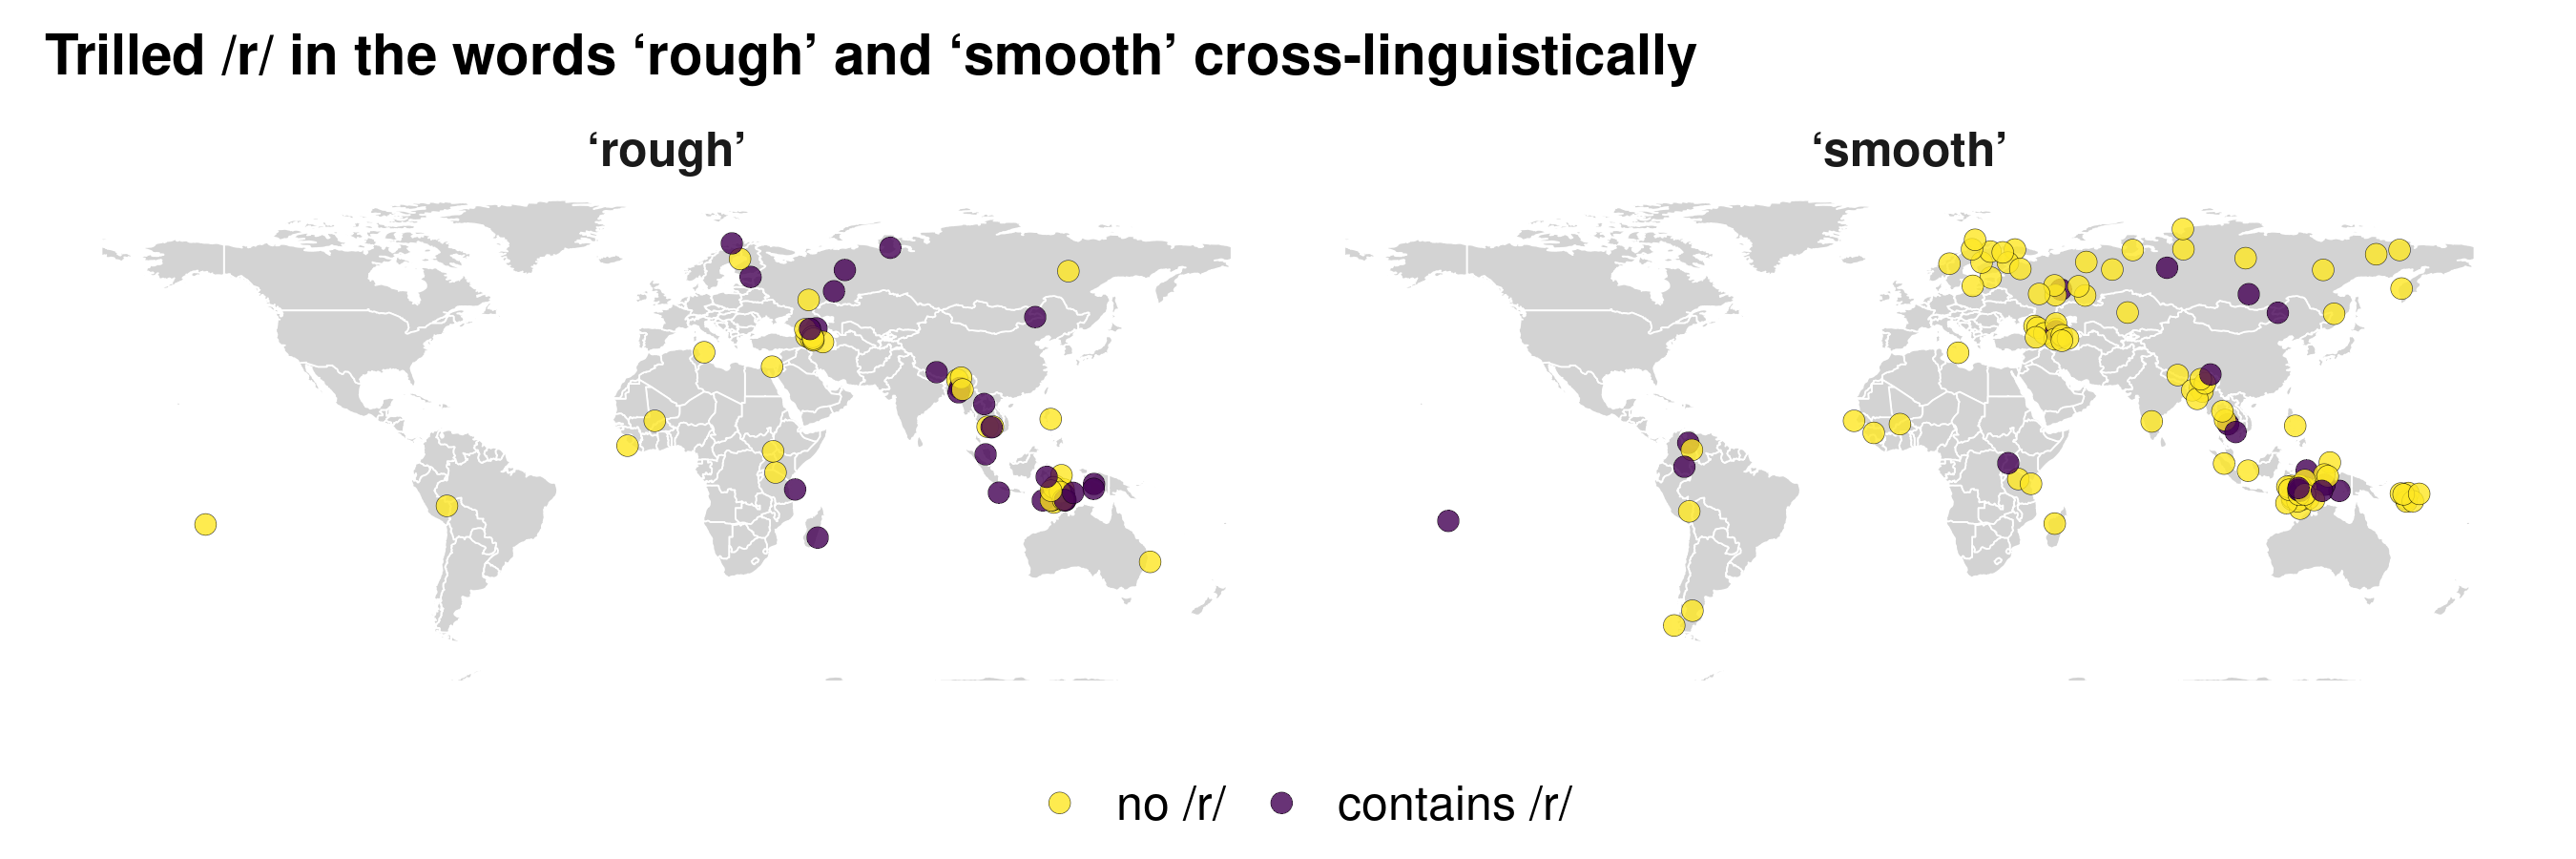
\includegraphics[width=1\linewidth, trim={0 0 0 1cm},clip]{substance/images/xling_map_revision}
	\caption[Distribution de la présence du /r/ trillé dans les termes \textg{rugueux} et \textg{lisse}]{Distribution de la présence du /r/ trillé dans les termes \textsc{rough} (\textg{rugueux}) et \textsc{smooth} (\textg{lisse}). Nous comparons les distributions de \textcite{winterTrilledAssociatedRoughness2022} (en haut) à la nôtre (en bas). Visuellement, il apparaît que dans l'étude d'origine et dans notre analyse, on retrouve plus de /r/ trillé associés à \textg{rugueux} plutôt qu'à \textg{lisse}.}
	\label{fig:xlingmap}
\end{figure}

%\begin{table}
%	\centering
%	\begin{tabular}{lcc}
%		\hline
%		& \textsc{trill} & \textsc{other} \\
%		\hline
%		\textg{Rugueux} avec /r/ & 37 & 27 \\
%		\textg{Rugueux} sans /r/ & 38 & 42 \\
%		\hline
%		\hline
%		\textg{Lisse} avec /r/ & 25 & 98 \\
%		\textg{Lisse} sans /r/ & 34 & 99 \\
%		\hline
%	\end{tabular}
%	\caption[A faire]{A faire}
%	\label{A faire}
%\end{table}

Nous avons utilisé les scripts \texttt{R} de \textcite{winterTrilledAssociatedRoughness2022} sans modification pour ajuster un modèle bayésien de régression logistique à effets mixtes pour prédire la présence du /r/.

Similairement au modèle de \citeauthor{winterTrilledAssociatedRoughness2022} (p. 8), nos prédicteurs fixes (\textg{\textit{fixed effect predictors}}) étaient la présence ou l'absence de /r/ trillé dans la langue, une variable binaire pour la rugosité (présence ou non d'un \textit{r}) et l'interaction de ces deux prédicteurs. Des ordonnées à l'origine aléatoires (\textg{\textit{random intercepts}}) pour les familles de langues et les aires linguistiques ont été incluses dans le but de contrôler pour ces facteurs, de même que des pentes aléatoires (\textg{\textit{random slopes}}) pour le /r/ trillé, la rugosité et leur interaction par famille et par aire. Comme il s'agit de vérifier que l'association est présente pour la rugosité à travers le terme \textsc{rough} (\textg{rugueux}), la présence de rhotique dans le terme \textsc{smooth} (\textg{lisse}) avait aussi été ajoutée. Nous avons utilisé les mêmes paramètres a priori présents dans l'analyse d'origine. Le but de notre réplication était de se concentrer sur les données et non les analyses statistiques.\\

La \autoref{fig:xlingmap} met en évidence la distribution des langues où l'on trouve les termes \textg{rugueux} et \textg{lisse} avec /r/ roulé. Notre analyse contient moins de données que l'analyse originale des auteurs, cependant vingt langues ont été recodées comme ayant un /r/ trillé. Le /r/ trillé semble visuellement plus présent dans le terme \textg{rugueux} que dans \textg{lisse}.\\

Initialement, les auteurs mentionnent dans leur article (p. 4) : \textg{[f]or languages with a trilled /r/, the estimated proportion of /r/ for the word ‘rough’ is 37\% [14\%, 61\%], while it is only 10\% [3\%, 19\%] for ‘smooth’, with an estimated difference of 27\% [6\%, 50\%] (with 99.7\% of posterior samples above zero [...])}, et \textg{27\% [12\%, 45\%] of rough words and 24\% [11\%, 41\%] of smooth words contain a rhotic, with an estimated difference of 2\% [–13\%, 19\%] (65.6\% of posterior samples above zero)}. Dans la \autoref{tab:propor_pred}, nous reportons les résultats issus de la réplication de leurs analyses ainsi que nos analyses après recodage des données.\\

\begin{table}
	\centering
	\begin{tabular}{p{2.8cm}p{1cm}p{2cm}p{1cm}p{2cm}}
		\hline
		& \multicolumn{2}{c}{\textsc{trill}} & \multicolumn{2}{c}{\textsc{other}}  \\
		\hline
		& \multicolumn{4}{c}{\textg{Rugueux}} \\
		Étude d'origine & 37\% & [14\%, 61\%] & 27\% & [12\%, 45\%] \\
		Notre analyse & 32\% & [10\%,  58\%] & 34\% & [16\%, 55\%] \\
		\hline
		& \multicolumn{4}{c}{\textg{Lisse}} \\
		Étude d'origine  & 10\% & [3\%, 19\%] & 24\% & [11\%, 41\%] \\
		Notre analyse  & 10\% & [3\%, 20\%] & 15\% & [6\%, 27\%] \\
		\hline
	\end{tabular}
	\caption{Proportions des prédictions des modèles avec les intervalles plausibles bayésiens à 95\% pour les mots \textg{rugueux} et \textg{lisse}.}
	\label{tab:propor_pred}
\end{table}

Pour notre analyse, pour les langues avec un /r/ trillé, la proportion estimée de /r/ pour le mot \textg{rugueux} est de 32\% [10\%, 58\%] alors que pour \textg{lisse} cette proportion estimée est de 10\% [3\%, 20\%], avec une différence estimée de 22\% [2\%, 46\%] (avec 98.4\% des échantillons postérieurs au-dessus de zéro). Pour les langues incluses sans /r/ trillé mais avec une autre rhotique, la proportion estimée de /r/ pour le mot \textg{rugueux} est de 34\% [16\%, 55\%] et pour \textg{lisse} la proportion est de 15\% [6\%, 27\%]. La différence estimée est de 19\% [2\%,36\%], (avec 98,65\% des échantillons postérieurs au-dessus de zéro) (\autoref{fig:xlingmodelpreds}). Que ce soit pour les /r/ trillés ou pour les autres types de /r/, nous observons des différences dans les proportions, suggérant que l'effet qui était absent pour les autres rhotiques dans l'article d'origine est présent avec notre re-codage des données.\\

Alors qu'il existe une interaction entre \textg{rugosité} et la présence du /r/ trillé dans l'analyse d'origine (1,53 en logarithme des probabilités de succès (\textg{\textit{log odds ratio}}) avec 98,9\% d'échantillons postérieurs supérieurs à zéro), notre analyse échoue à obtenir cette interaction entre \textg{rugosité} et la présence du /r/ trillé (0,37 en logarithme des probabilités de succès avec 83,5\% d'échantillons postérieurs supérieurs à zéro). Ce résultat peut s'expliquer car l'association n'est plus uniquement entre le /r/ trillé et \textg{rugosité}, mais bien entre toutes les rhotiques et \textg{rugosité}. Notre analyse permet de mettre en évidence que la \textg{rugosité} n'est pas associée uniquement avec le /r/ trillé mais aussi avec les autres rhotiques.

\begin{figure}
	\centering
	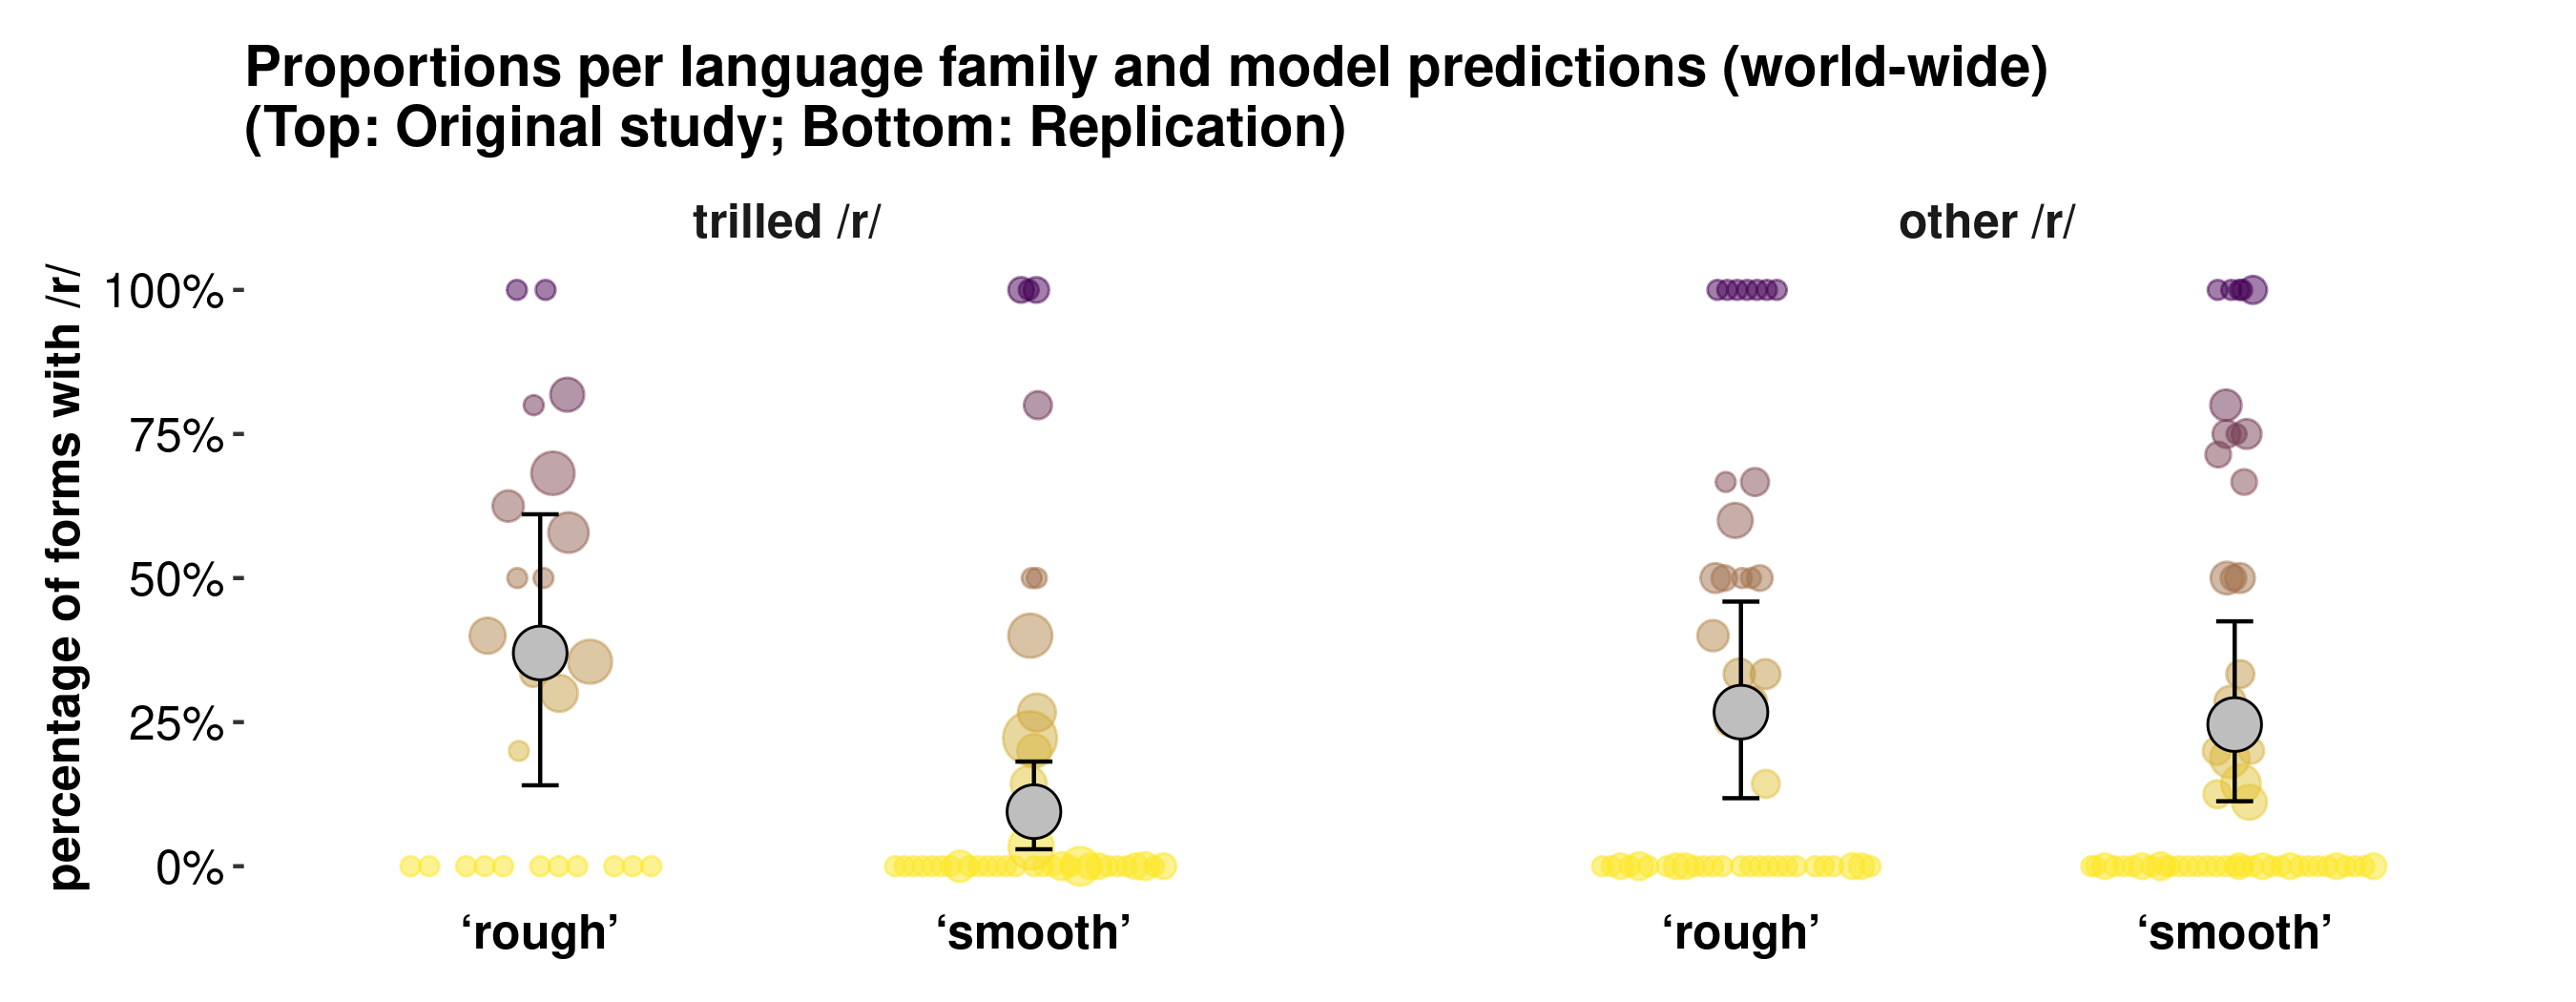
\includegraphics[width=1\linewidth, trim={0 0 0 0},clip]{substance/images/xling_model_preds}
	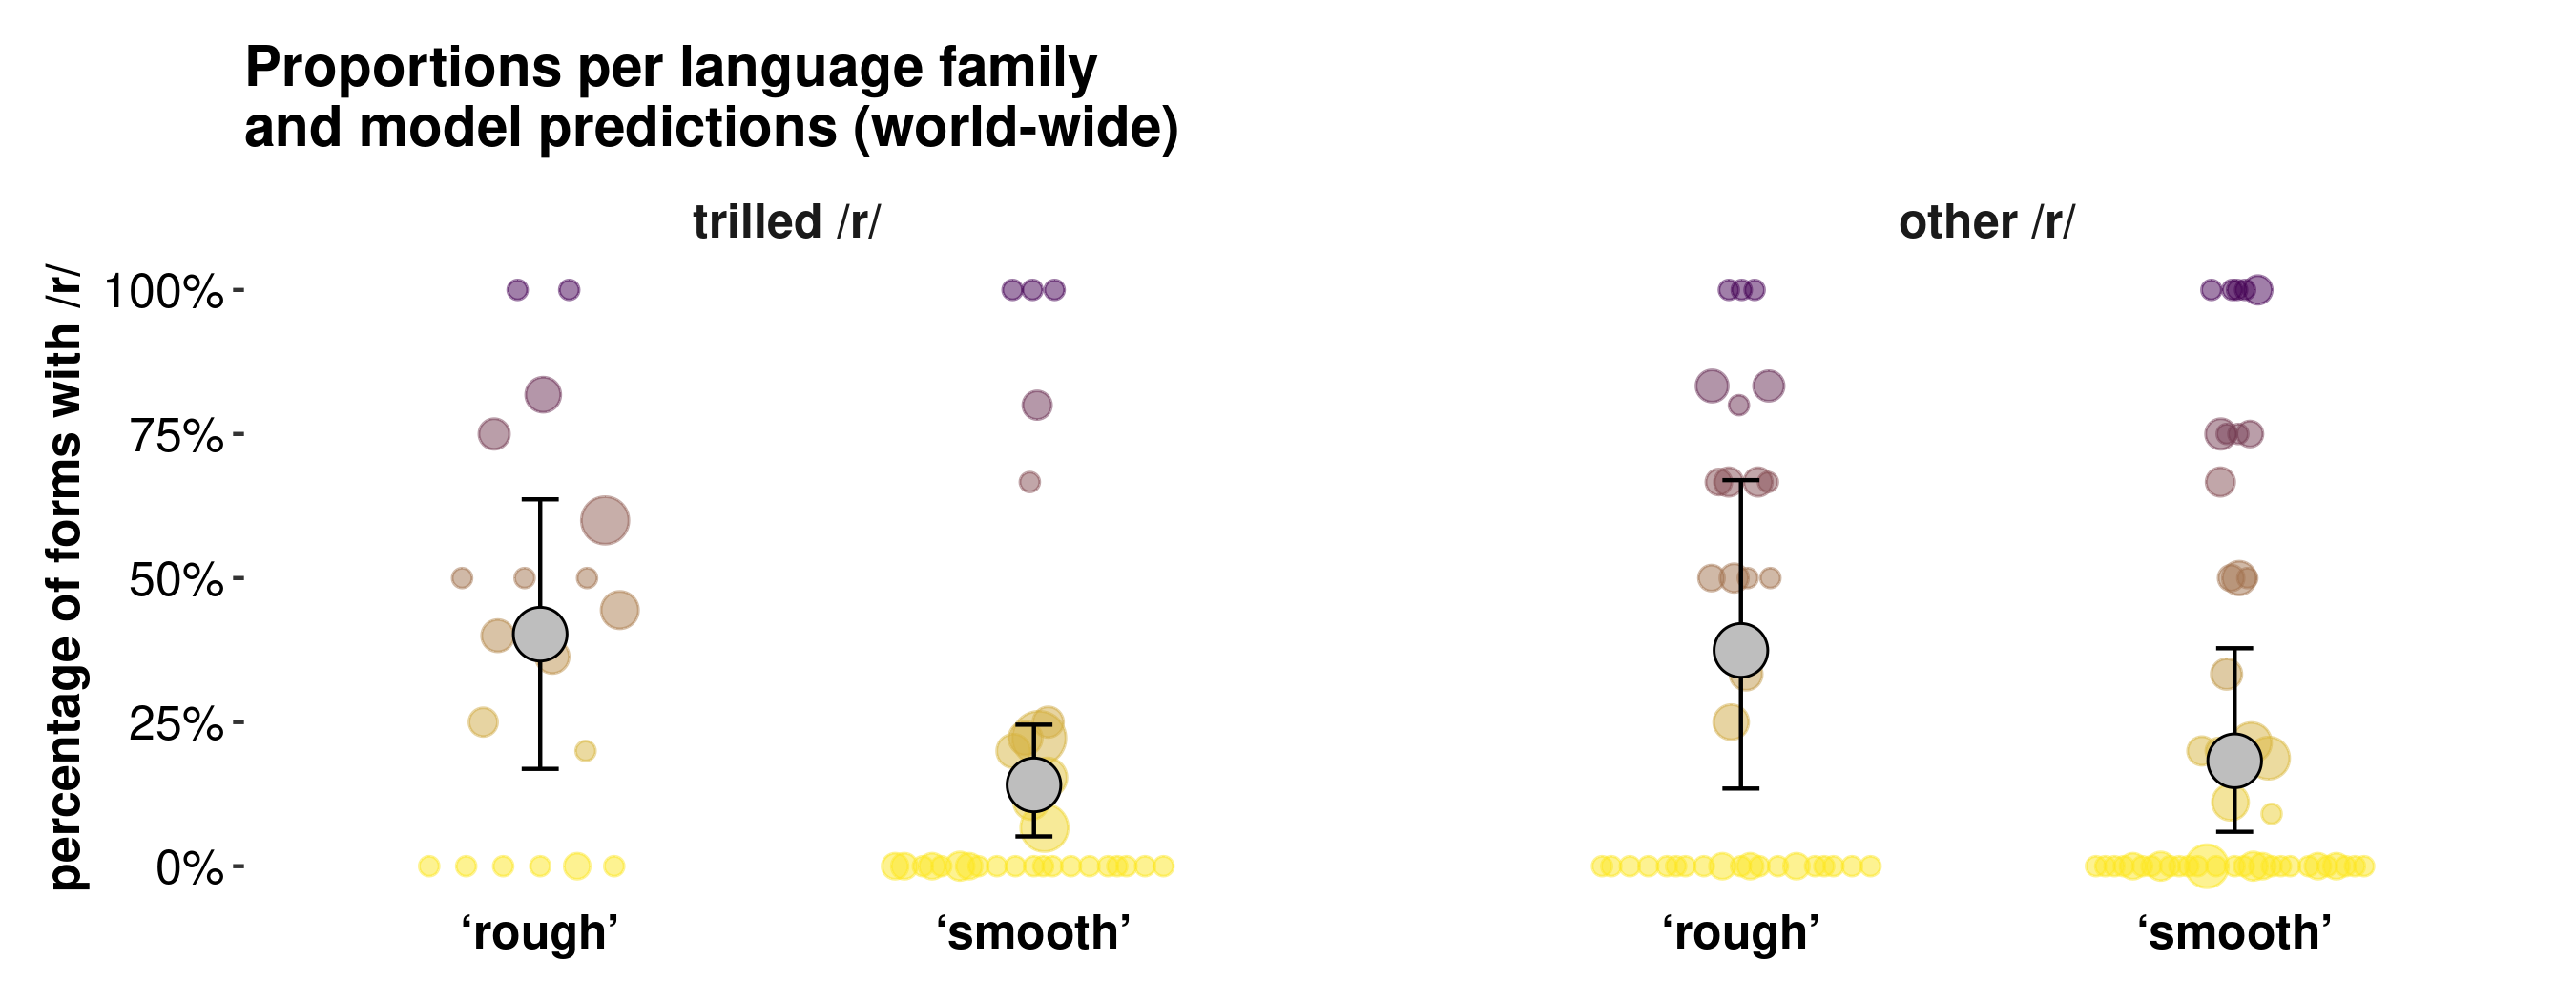
\includegraphics[width=1\linewidth, trim={0 0 0 1.5cm},clip]{substance/images/xling_model_preds_2}
	\caption[Graphique des prédictions du modèle de l'article d'origine et de notre réplication]{Graphique des prédictions du modèle de l'article d'origine et de notre réplication. À gauche : langues avec un /r/ trillé dans leur inventaire phonémique; à droite : langues avec un autre type de /r/. Les résultats sont agrégés par famille linguistique avec chaque point de couleur représentant une famille. La taille des cercles est proportionnelle au nombre de langues par famille. Les points gris sont les prédictions des modèles avec les intervalles plausibles bayésiens à 95\%.}
	\label{fig:xlingmodelpreds}
\end{figure}

\section{Discussion}

Pourquoi nous n'obtenons pas les mêmes résultats que \textcite{winterTrilledAssociatedRoughness2022} ?
L'hypothèse avancée par les auteurs pour expliquer cette différence suggère l'existence d'une réalisation tôtive de la rhotique qui aurait été trillée. Les auteurs parlent de \textg{left over from a past stage of the language} \parencite[3]{winterTrilledAssociatedRoughness2022}. Ce sont ensuite des pressions dues au coût du maintien de la conservation du segment, qui est articulatoirement complexe, qui font que la langue n'aurait pas maintenu le segment, qui reste néanmoins observable dans certains contextes, dans certains dialectes.
Cette hypothèse pourrait être étendue aux autres langues.
Nous pouvons supposer que les langues qui n'ont pas de trill synchroniquement (ou, du moins, pour lesquelles la réalisation de la rhotique n'est pas décrite comme trillée) sont passées par une étape où ce segment était trillé.
\textcite[22]{punnooseAuditoryAcousticStudy2010}, en se référant à Jones, mentionne que le trill peut être vu comme la source diachronique des autres rhotiques.
Comme les taps et les flaps sont aussi caractérisés par une modulation de l'amplitude, il est possible de supposer que ces segments permettent l'association avec la \textg{rugosité}. La modulation de l'amplitude est l'hypothèse de \textcite{winterTrilledAssociatedRoughness2022} pour expliquer l'association. En effet, cette modulation permet une \textg{auditory roughness} qui agit comme un attracteur culturel. Nous ne rentrons pas plus dans les détails et nous renvoyons les lecteurs/trices directement à l'article de \textcite{winterTrilledAssociatedRoughness2022} pour plus de détails.\\


Bien que le trill soit souvent associé aux reconstructions des réalisations des rhotiques, il faut être conscient  que la classe des rhotiques est une classe complexe avec énormément de variation. L'étude des trills à travers les grammaires et les systèmes de transcription force une interprétation unique de la réalisation du segment. C'est ce qui nous a posé problème avec cette étude cross-linguistique. Pour autant, des différentes grammaires que nous avons pu lire et des différentes sources que nous avons pu consulter, nous sommes convaincus qu'il existe des associations para-linguistiques avec le trill (cf. le trill en woisika \glotto{kama1365} utilisé pour montrer un trait expressif\footnote{Nous remercions Aleksandra Szczepańska pour son anecdote sur le \textg{prout} et le \textg{trill} en polonais où on retrouve un trill qui peut être allongé dans le mot.}) et que le trill peut se trouver dans la langue sans pour autant avoir une fonction linguistique.

\begin{displayquote} 
	
Extrait de \textit{Woisika II: phonemics} par \parencite[102--103]{stokhofWoisikaIIPhonemics1979}:
\begin{exe}  
	\ex EXPRESSIVE FEATURES
	\begin{xlistn} \label{ex:chicken}
		\item Quantity and aspiration (with facultative breathiness) may create emphasis or indicate the speaker's emotional attitude.\\	
		A very long apical trill (in free variation with normal [r, r̪]) is produced in words such as:\\
		\textrm{[ar$:$]}, [tar$:$], [dar$:$] and [kur$:$]
		The first three are onomatopoeias and express the vibration of string and bow immediately after the release of the tension, i.e. when the arrow has been fired.\\
		\textrm{[kur$:$]} or more often /'kurkurkur/ (with normal /r/) is a call note for chickens.
	\end{xlistn}
\end{exe}

\end{displayquote}

Du fait de la variation du trill et du problème des transcriptions, il faut souligner que la réalisation du trill comme telle reste conditionnée par des facteurs comme sa position dans le mot, ou le contexte de production. Le trill est en variation avec d'autres allophones. De ce fait, il n'y a aucune garantie que dans les mots pour \textg{rugueux} pris en compte par \textcite{winterTrilledAssociatedRoughness2022} les <r> soient réalisés comme des trills. Nous remarquons que dans certaines transcriptions issues de CLICS, il y a eu une réinterprétation de segments dérivés du <r> comme \textit{ɹ} en un trill [r].
En conclusion, l'association entre \textg{trill} et \textg{rugosité} peut exister. Néanmoins, nous suggérons que la présence de /r/ trillés dans les langues doit être cherchée en dehors des inventaires phonémiques.
Dans le chapitre suivant, nous proposerons une réflexion sur la place des sons dans les grammaires et dans l'élaboration des grammaires.